\documentclass[border=3pt]{standalone}
% Preâmbulo compartilhado pelos diagramas TikZ da aula
\usepackage[T1]{fontenc}
\usepackage[utf8]{inputenc}
\usepackage{lmodern}
\usepackage{amsmath}
\usepackage{xcolor}
\usepackage{tikz}
\usetikzlibrary{arrows.meta,angles,quotes,decorations.pathmorphing,calc,
                positioning,shapes.geometric,backgrounds,fit}

% Paleta (mesma dos SVGs originais)
\definecolor{dblue}{HTML}{2A5B8C}
\definecolor{dorange}{HTML}{B3541E}
\definecolor{dgreen}{HTML}{4A7C59}
\definecolor{dred}{HTML}{9C4B4B}
\definecolor{dcream}{HTML}{F4F1EA}
\definecolor{dshade}{HTML}{DDD7C9}

% Estilos comuns (prefixo d... para não colidir com chaves internas do pgf)
\tikzset{
  >={Stealth[length=2mm]},
  dguide/.style={gray!55, dashed, line width=0.4pt},
  daxis/.style={gray!60, line width=0.7pt, ->},
  dbody/.style={fill=black!3, draw=black!80, line width=1pt},
  dacc/.style={draw=dblue, line width=1pt},
  dlbl/.style={black!55, font=\small},
  dsub/.style={black!45, font=\footnotesize},
  dstate/.style={circle, draw=black!80, fill=dcream, line width=1pt,
                 minimum size=17mm, font=\large, inner sep=1pt},
  dobs/.style={circle, draw=black!80, fill=dshade, line width=1pt,
               minimum size=14mm, font=\large, inner sep=1pt},
  dbox/.style={rounded corners=2pt, draw=black!80, fill=dcream, line width=1pt,
               align=center, inner sep=6pt},
  dtrans/.style={->, dblue, line width=1pt},
  dmeas/.style={->, dorange, line width=1pt},
}

\begin{document}
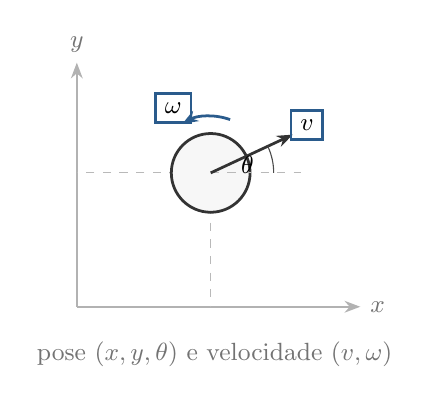
\begin{tikzpicture}[scale=1]

  % eixos de coordenadas
  \draw[daxis] (0,0) -- (3.6,0) node[right, dlbl] {$x$};
  \draw[daxis] (0,0) -- (0,3.1) node[above, dlbl] {$y$};

  % posição do robô
  \coordinate (R) at (1.7,1.7);

  % guias tracejadas
  \draw[dguide] (R) -- (1.7,0);
  \draw[dguide] (R) -- (0,1.7);

  % corpo do robô
  \draw[dbody] (R) circle (0.5);

  % linha de referência e direção (heading)
  \draw[dguide] (R) -- ++(1.15,0) coordinate (ref);
  \draw[->, black!80, line width=1pt] (R) -- ++(25:1.15) coordinate (head);

  % ângulo theta
  \pic[draw=black!70, angle radius=8mm, "$\theta$" {black, font=\small}]
      {angle = ref--R--head};

  % velocidade linear v (na ponta do heading)
  \node[dacc, font=\small] at ($(head)+(0.18,0.12)$) {$v$};

  % velocidade angular omega (arco azul)
  \draw[dacc, ->] ([shift=(70:0.72)]R) arc (70:120:0.72);
  \node[dacc, font=\small] at ($(R)+(120:0.95)$) {$\omega$};

  % legenda
  \node[dlbl] at (1.75,-0.6) {pose $(x,y,\theta)$ e velocidade $(v,\omega)$};

\end{tikzpicture}
\end{document}
